\documentclass[tikz,border=7pt]{standalone}
\begin{document}
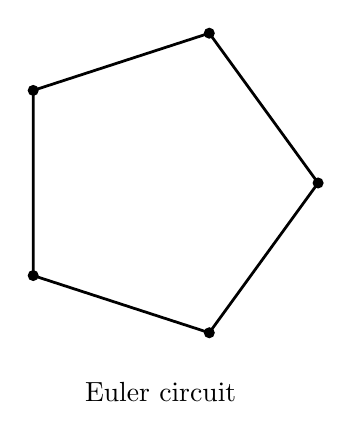
\begin{tikzpicture}[line width=1pt]
\foreach \a in {0,72,...,288} \coordinate (v\a) at (\a:2);
\draw (v0)--(v72)--(v144)--(v216)--(v288)--cycle;
\foreach \a in {0,72,...,288} \fill (v\a) circle (2pt);
\node at (0,-2.65) {Euler circuit};
\end{tikzpicture}
\end{document}
